\documentclass[12pt]{article}
\usepackage[UTF8]{ctex}

\usepackage{geometry}
\geometry{left=2.5cm, right=2.5cm, top=2.5cm, bottom=2.5cm}

\usepackage{graphicx}
\graphicspath{ {./images/} }

\makeatletter
\def\verbatim@font{\linespread{0.85}\normalfont\ttfamily}
\makeatother

\begin{document}

\title{同化棋 (Ataxx) 实验报告}
\author{天音あめ}
\date{2021 年 12 月 1 日}

\maketitle

% \centerline{测试文本}
\begin{verbatim}
                            +------------------+
                            | Welcome to Ataxx |
                            +------------------+
                            | 1. New Game      |
                            | 2. Save Game     |
                            | 3. Load Game     |
                            | 4. Quit          |
                            +------------------+
                            Enter your choice: 
\end{verbatim}

\newpage

\section{功能介绍}

\begin{itemize}
    \item 纯 ASCII 字符绘制界面, 并采用输入起始坐标 $\mathrm Ax$ 与目标坐标 $\mathrm By$ 的方式进行移动.
    \begin{verbatim}
                            Round 012
    07 O=======------------------------------------------|
       |------------------------------------=============X 13
                    1   2   3   4   5   6   7
                  +---+---+---+---+---+---+---+
                A |   | X | X | X | X |   |   |
                  +---+---+---+---+---+---+---+
                B | X | X | X | O | X | X |   |
                  +---+---+---+---+---+---+---+
                C | X | O | O | O | X |   |   |
                  +---+---+---+---+---+---+---+
                D | X | O | O |   |   |   |   |
                  +---+---+---+---+---+---+---+
                E |   |   |   |   |   |   |   |
                  +---+---+---+---+---+---+---+
                F |   |   |   |   |   |   |   |
                  +---+---+---+---+---+---+---+
                G | X |   |   |   |   |   | O |
                  +---+---+---+---+---+---+---+
                          Your(O') turn
    Enter Ax By to move your chess (ZZ for quit, RR for regret): \end{verbatim}
    任意时刻可以使用 \texttt{RR} \textbf{悔棋}, 或者使用 \texttt{ZZ} 返回主界面. \\
    棋盘上方实时显示当前回合数与棋子数比分, 棋盘下方实时显示游戏状态. \\
    移动棋子后, 会有\textbf{动画}显示棋子移动与棋子翻转的过程.

    \item 拥有双人对战与人机对战两种模式, 人机模式可选难度.
    \begin{verbatim}
    +---------------+
    |   Game Type   |
    +---------------+
    | 1. VS CPU Lv1 |
    | 2. VS CPU Lv2 |
    | 3. VS CPU Lv3 |
    | 4. VS Player  |
    | 5. Return     |
    +---------------+
    Enter your choice: \end{verbatim}

    \item 机器算法优秀, \textbf{在 Botzone (ID : \texttt{6199248863626007396249c0}) 上获得 2100+ 分}, 可以在 1 秒内完成决策. 因笔者本人棋力水平有限, 甚至无法在 VS CPU Lv1 中获胜.

    \newpage

    \item 支持保存当前的游戏进度, 或者读取已保存的进度, 并能同时拥有最多 5 个存档.
    \begin{verbatim}
    +-----+---------------+-------+--------------------------+
    | No. |     Rival     | Score |           Time           |
    +-----+---------------+-------+--------------------------+
    |  1  | VS CPU(X) Lv3 | 07:13 | Sun Nov 21 01:16:57 2021 |
    |  2  |               |       |        Empty slot        |
    |  3  |   VS Player   | 20:17 | Sat Nov 20 20:02:31 2021 |
    |  4  |               |       |        Empty slot        |
    |  5  |               |       |        Empty slot        |
    +-----+---------------+-------+--------------------------+
    Enter your slot number (0 for cancel): \end{verbatim}
\end{itemize}

\section{代码实现}

\begin{tabular}{|l|l|}
\hline \texttt{main.cpp} & 主程序部分, 包含主界面逻辑 \\
\hline \texttt{ai.hpp} & 包含人机对战下的自动决策部分 \\
\hline \texttt{chessboard.hpp} & 包含棋盘类, 保存棋盘的状态与估价 \\
\hline \texttt{file.hpp} & 包含保存进度与读取进度相关文件操作 \\
\hline \texttt{game.hpp} & 包含游戏回合逻辑, 同时处理双人对战与人机对战 \\
\hline \texttt{gamestate.hpp} & 包含游戏进度类, 保存当前游戏的完整状态 \\
\hline \texttt{os.hpp} & 包含清屏, 延时等平台相关部分 \\
\hline \texttt{pos.hpp} & 包含对棋子位置移动的判断处理 \\
\hline \texttt{scanner.hpp} & 包含输入部分, 从玩家处获取格式正确输入 \\
\hline \texttt{ui.hpp} & 包含棋盘, 存档列表等界面绘制部分 \\
\hline
\end{tabular}
\\

\indent 考虑到文件数目不多, 每次均重新构建目标文件的时间可以接受. \\
\indent 所以把定义均放置在了 \texttt{.hpp} 内而没有独立 \texttt{.cpp}, 并且没有编写 Makefile. \\
\indent 编译整个程序只需要 \texttt{g++ main.cpp -O2 -o main} 即可.

\newpage

\section{算法实现}

\begin{figure}[h]
    \centering
    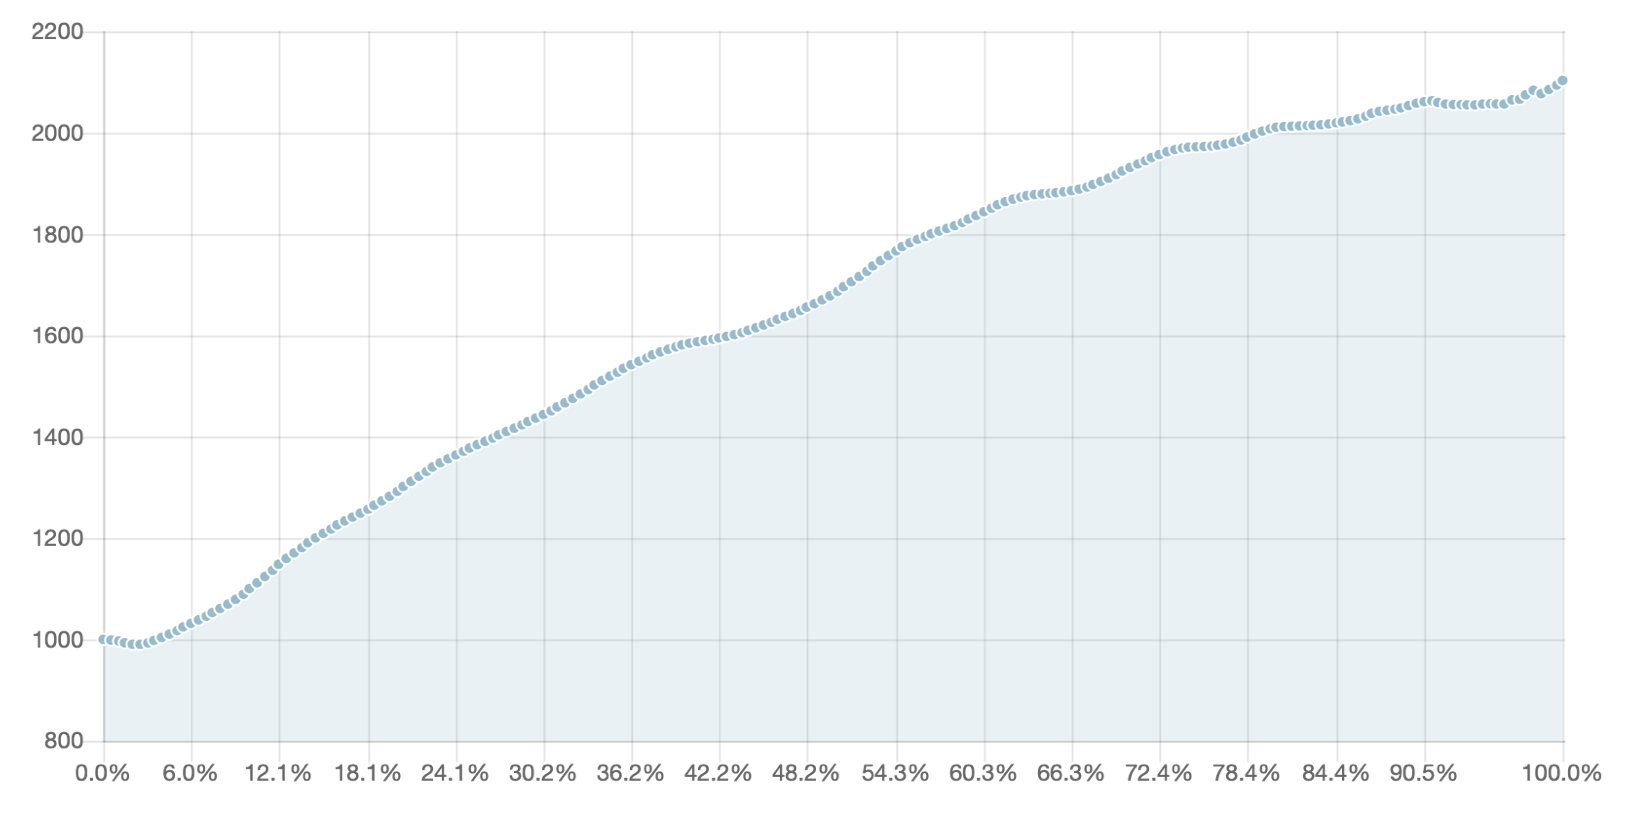
\includegraphics[width=\textwidth]{rank}
    \caption{\texttt{6199248863626007396249c0} 在 Botzone 上的总趋势 (截至 2021-12-01 21:58:05)}
\end{figure}

\indent 目前该算法在 Botzone 天梯\footnote{\texttt{https://botzone.org/game/ranklist/5809c7647f65182b044b5e3b\#6199248863626007396249c0}.}上稳定在前 10 名. \\
\indent 算法基于 Minimax 搜索\footnote{\texttt{https://en.wikipedia.org/wiki/Minimax}.}配合 Alpha-Beta 剪枝\footnote{\texttt{https://en.wikipedia.org/wiki/Alpha-beta\_pruning}.}.

\begin{itemize}
    \item 棋盘大小 $7 \times 7 = 49 \leq 64$, 使用两个无符号 64 位整数, 分别表示白子与黑子的位置即可保存棋盘, 没有必要使用数组. 这样不仅在复制棋盘时更快, 获取棋子可移动的位置之类的操作也只需要做 bitwise AND 运算.
    \item 棋子移动到八连通的位置时, 自身不会消失. 所以在考虑八连通决策时, 不应该考虑每个棋子可以移动到哪个空地, 而应该考虑每个空地\textbf{是否可以}被某个棋子移动到. 这样可以减少大量重复决策状态.
    \item 笔者测试了大量不同的棋盘估价函数, 最后结论为最优估价函数为己方棋子数减去敌方棋子数. 造成这个结论的原因猜测为, 计算棋子数只需要使用 \texttt{popcountll} 计数二进制 \texttt{1} 的个数, 非常迅速, 所以 Minimax 搜索能搜索更多层. \\ 当然, 要注意判断必胜与必败的情况 (棋盘满, 一方无子, 或一方不能移动).
    \item Minimax 搜索层数不易估计, 因此采取迭代加深\footnote{\texttt{https://en.wikipedia.org/wiki/Iterative\_deepening\_depth-first\_search}.}的搜索方式. 每次搜索返回最优解后, 便将允许的搜索深度加一. 因为要在 1 秒内决策完成, 这同时也方便了时间的控制, 只需要在加层时判断是否接近 1 秒, 并在 Minimax 搜索时若接近 1 秒则立刻终止.
    \item 对于 Alpha-Beta 剪枝而言, 搜索子树的顺序非常重要. 笔者采取了一种类似 Principal variation search (又称 NegaScout) 算法\footnote{\texttt{https://en.wikipedia.org/wiki/Principal\_variation\_search}.}的方式决定顺序, 但考虑到保存大量子树结点搜索顺序开销巨大, 所以并没有使用 NegaScout 的零窗口搜索. \\ 最后的决策只关心第一步的移动, 并且第一步的子树也最大, 在越浅层成功 Alpha-Beta 剪枝则效率越高. 所以对于一次深度为 $D$ 的 Minimax 搜索, 先对所有可能的第一步移动进行一次深度为 $\left\lfloor \frac{D}{2} \right\rfloor$ 的 Minimax 搜索, 并将第一步移动按照搜索估价排序. 在这之后, 再按照排序后的顺序进行深度为 $D$ 的搜索. 这样牺牲了若干次深度为 $\left\lfloor \frac{D}{2} \right\rfloor$ 的搜索, 但却能使深度为 $D$ 的搜索剪去更多的分枝, 实际效率提升显著. \\ 更进一步, 在迭代加深过程中, 深度为 $D - 1$ 时的最优决策也是可以利用的. 这个最优决策在深度为 $D$ 时, 保持仍为最优决策的概率比被其它决策取代它的概率要大. 所以可以在排序第一步时, 把上一次的最优决策提至最前, 如此又可以剪去另一批子树.
\end{itemize}

\section{总结与展望}

\indent 本同化棋实验项目简要实现了字符绘制界面并使用 CLI 交互, 有专门的输入处理类, 对用户输入的容错性好. 同时配合平台相关的清屏与延时等 API, 也实现了棋子移动的动画效果, 用户观感更加舒适并更加易于理解. 配合标准的二进制文件读写功能, 实现了游戏局面的随时存盘与复盘. 除此之外, 本项目也拥有相对完善的机器决策功能, 能够在人机对决乃至 Botzone 上的机机对决中保持一个较高的胜率. \\
\indent 考虑到纯 C++ 实现图形界面不易, 因此本项目没有完成 GUI 交互. 但通过 Qt 等现代化的跨平台 UI 库, 也可以比较容易地将本项目改造为 GUI 项目. 甚至考虑到代码逻辑清晰, 文件之间耦合度低, 将整个项目逻辑部分使用 JavaScript 重写并用 HTML/CSS 制作 GUI, 从而将本项目放置到网页上运行也不是什么难事. 本项目后续将在 GitHub 上开源, 欢迎各位在此基础上加以改造, 做出更加用户友好, 机器决策更加强大的同化棋项目.

\end{document}
